\documentclass{beamer}

\usetheme{Madrid}
\usecolortheme{default}
\usepackage{xcolor}
\AtBeginSection[]{
  \begin{frame}{Outline}
    \tableofcontents[currentsection]
  \end{frame}
}
\title{Statistical Analysis Discussion}
\date{\today}

\begin{document}

\begin{frame}
	\titlepage
\end{frame}


\section{``tximport"}
\begin{frame}
    \frametitle{``tximport" or not?}
	\begin{itemize}
        \item My proposal: Just round the salmon decimals and be done with it.
        \item What does tximport do? Round it also but take into account different isoform usage (?)
    \end{itemize}
\end{frame}

\section{ANOVA Basics}
\begin{frame}
\frametitle{ANOVA Basics: Dummy coding}

Consider 2 treatments and $n$ observations.
\[
\begin{bmatrix}
y_{1} \\
y_{2} \\
\vdots \\
y_{n_1} \\
\textcolor{red}{y_{n_1+1}} \\
\vdots \\
\textcolor{red}{y_{n}}
\end{bmatrix}
=
\begin{bmatrix}
1 & 0 \\
1 & 0 \\
\vdots & \vdots \\
1 & 0 \\
1 & \textcolor{red}{1} \\
\vdots & \vdots \\
1 & \textcolor{red}{1}
\end{bmatrix}
\begin{bmatrix}
\beta_0 \\
\textcolor{red}{\beta_1}
\end{bmatrix}
+
\begin{bmatrix}
\epsilon_{1} \\
\epsilon_{2} \\
\vdots \\
\epsilon_{n_1} \\
\epsilon_{n_1+1} \\
\vdots \\
\epsilon_{n}
\end{bmatrix}
\]
\\~\\
\footnotesize
The parameter value $\textcolor{red}{\beta_1}$ is the \textbf{change with respect to basline (control)} $\beta_0$. It will have an assigned p-value, which corresponds (under certain conditions) to a simple t-test.
   
\end{frame}


\begin{frame}[fragile]{ANOVA Basics: What is a Design Matrix $\mathbf{X}$?}

\begin{block}{Definition}
The design matrix $\mathbf{X}$ is a structured array that translates categorical factors and continuous variables into numerical predictors for a linear model ($\mathbf{y} = \mathbf{X}\boldsymbol{\beta} + \boldsymbol{\epsilon}$).
\end{block}

\vspace{0.3em}
\small
\textbf{Example:} 3 Treatments ($T_1$ ref, $T_2, T_3$) $\times$ 2 Time Points ($t_1$ ref, $t_2$) with interaction:

\[
\begin{bmatrix}
y_{T1, t1} \\ y_{T1, t2} \\ y_{T2, t1} \\ y_{T2, t2} \\ y_{T3, t1} \\ y_{T3, t2}
\end{bmatrix}
=
\begin{bmatrix}
1 & 0 & 0 & 0 & 0 & 0 \\
1 & 0 & 0 & 1 & 0 & 0 \\
1 & 1 & 0 & 0 & 0 & 0 \\
1 & 1 & 0 & 1 & 1 & 0 \\
1 & 0 & 1 & 0 & 0 & 0 \\
1 & 0 & 1 & 1 & 0 & 1
\end{bmatrix}
\begin{bmatrix}
\beta_0 \\ \beta_{T2} \\ \beta_{T3} \\ \beta_{\text{time}} \\ \beta_{T2:\text{time}} \\ \beta_{T3:\text{time}}
\end{bmatrix}
+
\begin{bmatrix}
\epsilon_1 \\ \epsilon_2 \\ \epsilon_3 \\ \epsilon_4 \\ \epsilon_5 \\ \epsilon_6
\end{bmatrix}
\]

\footnotesize
\textbf{Columns:} Intercept | $T_2$ dummy | $T_3$ dummy | Time dummy | $T_2 \times \text{Time}$ | $T_3 \times \text{Time}$
\end{frame}

\section{Negative Binomial GLM Basics}

\begin{frame}[fragile]{Count Data \& The Negative Binomial Model}

\begin{block}{The Nature of RNA-Seq Count Data}
Read counts ($K_{ij}$) are \textbf{non-negative integers} representing gene expression levels (sum of all fragments mappped to a gene).
\end{block}

\vspace{0.3em}
\begin{itemize}
    \item \textbf{Why not standard Linear Regression?} Assumes continuous, normally distributed errors, which fails for zero-heavy, highly skewed count data.
    \item \textbf{Why not Poisson?} Poisson assumes $\text{variance} = \text{mean}$. Real biological replicates show \textbf{overdispersion} ($\text{variance} > \text{mean}$).
    \item \textbf{The Solution (Negative Binomial):} 
    Extends Poisson by adding a gene-specific dispersion parameter ($\alpha_i$) to account for biological and technical variability:
    \[
    \text{Var}(K_{ij}) = \mu_{ij} + \alpha_i \mu_{ij}^2
    \]
\end{itemize}

\end{frame}

\begin{frame}[fragile]{Generalized Linear Model (GLM) for $K_{ij}$}

\small
\textbf{Definition of terms:}
\begin{itemize}
    \item $K_{ij}$: Read count for gene $i$ in sample $j$ ($K_{ij} \in \mathbb{N}_0$)
    \item $s_{ij}$: Size factor: \textbf{accounting for sequencing depth differences} (Median of Ratios normalization!!)
    \item $\mu_{ij}$: Expected mean parameter of the Negative Binomial ($\mu_{ij} \in \mathbb{R}^+$)
\end{itemize}

\vspace{0.2em}
\textbf{The GLM Framework:}
\[
K_{ij} \sim \text{NB}(\text{mean} = \mu_{ij}, \text{dispersion} = \alpha_i)
\]
\[
\mu_{ij} = s_{ij} q_{ij}
\]
\\~\\
The dispersion parameter $\alpha_i$ is estimated also, in a very smart way pooling information from all genes. We do not get into that, we assume it constant.

\end{frame}


\begin{frame}{The negative binomial model for counts}

Read count of gene $i$ in sample $j$:
\[
    K_{ij} \sim \text{NB}\big(\textcolor{red}{\mu_{ij}},\, \textcolor{blue}{\alpha_i}\big)
\]

Probability mass function (scary looking, but you don't need to care about it):
\[
    P(K_{ij}=k) =
    \binom{k + 1/\textcolor{blue}{\alpha_i} - 1}{k}
    \left(\frac{1}{1 + \textcolor{blue}{\alpha_i} \textcolor{red}{\mu_{ij}}}\right)^{1/\textcolor{blue}{\alpha_i}}
    \left(\frac{\textcolor{blue}{\alpha_i} \textcolor{red}{\mu_{ij}}}{1 + \textcolor{blue}{\alpha_i} \textcolor{red}{\mu_{ij}}}\right)^{k}
\]

\vspace{0.2em}
\centering
\alert{What we care about: $\mu$ is the expected count in each group}

\end{frame}
\begin{frame}
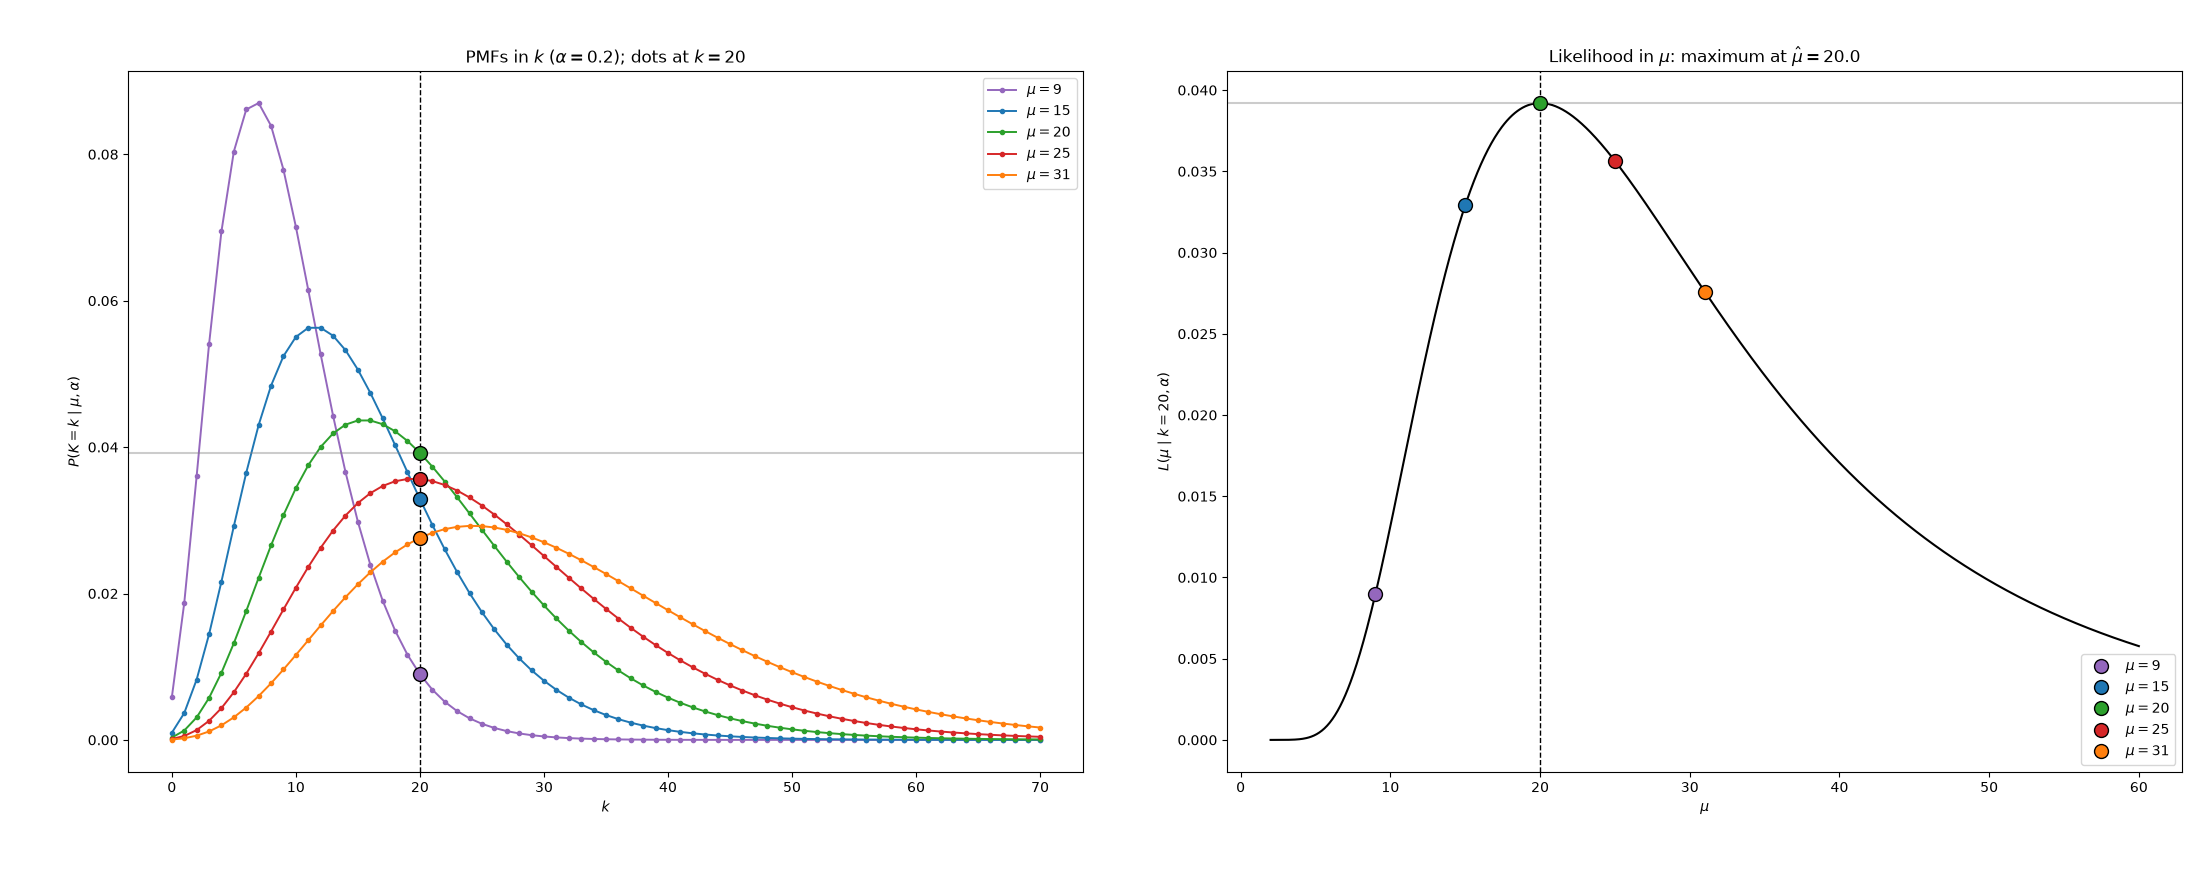
\includegraphics[width=\textwidth]{plots/NB.png}
\end{frame}

\begin{frame}
\frametitle{From ANOVA to counts: the DESeq2 model}

Count of gene $i$ in sample $j$: $K_{ij}\sim \text{NB}(\mu_{ij},\alpha_i)$ with
\[
    \mu_{ij} = s_jq_{ij} \iff \frac{\mu_{ij}}{s_j} = q_{ij}
    \qquad\text{and}\qquad    
\log_2 q_{ij} = \sum_r x_{jr}\beta_{ir} = \mathbf{x}_j^\top\boldsymbol\beta_i
\]
\vspace{0.2cm}
\begin{block}{Depth-Normalized Abundance}
    \[
\log_2 q_{ij} = \log_2(\frac{\mu_{ij}}{s_j})
    \]
    \textbf{Interpretation:} This represents the expected abundance of gene $i$ in sample $j$, and it is the part that directly depends on your experiment design matrix $X$.
\end{block}
\vspace{0.2cm}
We are "predicting" the $\log_2$ of the depth normalized counts!
\end{frame}

\begin{frame}
\frametitle{From ANOVA to counts: the DESeq2 model}
\vspace{0.3em}
\[
\begin{bmatrix}
\log_2 q_{i1} \\
\vdots \\
\log_2 q_{in_1} \\
\textcolor{red}{\log_2 q_{i,n_1+1}} \\
\vdots \\
\textcolor{red}{\log_2 q_{in}}
\end{bmatrix}
=
\begin{bmatrix}
1 & 0 \\
\vdots & \vdots \\
1 & 0 \\
1 & \textcolor{red}{1} \\
\vdots & \vdots \\
1 & \textcolor{red}{1}
\end{bmatrix}
\begin{bmatrix}
\beta_{i0} \\
\textcolor{red}{\beta_{i1}}
\end{bmatrix}
\]

\vspace{0.2em}
\begin{tabular}{lll}
Control: & $q_{ij} = 2^{\beta_{i0}}$ & baseline normalized count \\
Treated: & $q_{ij} = 2^{(\beta_{i0} + \textcolor{red}{{\beta_{i1}}})} = 2^{\beta_{i0}}\,\textcolor{red}{2^{\beta_{i1}}}$ & baseline $\times$ \textcolor{red}{fold change} \\
\end{tabular}

\vspace{0.1em}
\normalsize
\begin{align*}
\log_2\text{FC}
&= \log_2\frac{q_{\text{treated}}}{q_{\text{control}}}
= \log_2\frac{2^{\beta_{i0}+\beta_{i1}}}{2^{\beta_{i0}}}
= \log_2\frac{2^{\beta_{i0}}\,2^{\beta_{i1}}}{2^{\beta_{i0}}} \\[0.4em]
&= \log_2 2^{\beta_{i1}} = \textcolor{red}{\beta_{i1}}
\end{align*}
$\beta_{i1}=1$: the normalized count doubles; $\beta_{i1}=-1$: it halves.
\end{frame}

\section{Interpreting \texttt{$\sim$ treatment * time * temperature}}
% ---------- Slide 1: setup ----------
\begin{frame}
\frametitle{Interpreting \texttt{treatment * time * temperature}: setup}

\begin{block}{Reference (baseline) condition}
mock, \quad $t = 0.5$, \quad 21$^\circ$C
\end{block}

\vspace{0.3cm}
Each factor becomes a 0/1 indicator \textbf{relative to the reference}:
\begin{itemize}
    \item $T = 1$: treated (0 = mock)
    \item $t = 1$: later time (0 = 0.5)
    \item $H = 1$: other temperature (0 = 21$^\circ$C)
\end{itemize}

\vspace{0.3cm}
The model has 8 coefficients (intercept, 3 main effects, 3 two-way and 1 three-way interaction):
\[
\log_2 q_{ij} = \beta_0 + \beta_T T + \beta_t t + \beta_H H
+ \beta_{Tt}\,Tt + \beta_{TH}\,TH + \beta_{tH}\,tH + \beta_{TtH}\,TtH
\]

\vspace{0.1cm}
\alert{Every coefficient is a $\log_2$ change relative to a specific condition.}
\end{frame}

% ---------- Slide 2: main effects ----------
\begin{frame}
\frametitle{Baseline and main effects}

\renewcommand{\arraystretch}{1.6}
\begin{tabular}{@{}ll@{}}
$\beta_0$ & $\log_2$ normalized count in the \textbf{reference} (mock, 0.5, 21$^\circ$C) \\
$\beta_T$ & treatment LFC vs mock, \textbf{only} at $t=0.5$ and 21$^\circ$C \\
$\beta_t$ & time effect, \textbf{only} in mock at 21$^\circ$C \\
$\beta_H$ & temperature effect, \textbf{only} in mock at $t=0.5$ \\
\end{tabular}

\vspace{0.5cm}
\begin{block}{Warning}
With interactions in the model, a ``main effect'' is the effect \textbf{at the reference level of the other factors}. It is not the overall effect of the treatment.
\end{block}
\end{frame}

% ---------- Slide 3: interactions ----------
\begin{frame}
\frametitle{Interactions: how an effect changes}
\small
\renewcommand{\arraystretch}{1.6}
\begin{tabular}{@{}ll@{}}
$\beta_{Tt}$ & \textbf{change in the treatment LFC} at the later time (at 21$^\circ$C) \\
$\beta_{TH}$ & \textbf{change in the treatment LFC} at the other temperature (at $t=0.5$) \\
$\beta_{tH}$ & change in the time effect at the other temperature (in mock) \\
$\beta_{TtH}$ & change in $\beta_{Tt}$ at the other temperature (a ``difference of differences'') \\
\end{tabular}

\end{frame}

% ---------- Slide 4: LFC per condition ----------
\begin{frame}
\frametitle{Treatment vs mock in each condition}

In the treated-minus-mock difference, every term without $T$ cancels, exactly as in the $\beta_{i1}$ derivation:
\[
\log_2\text{FC}_{(t,H)} = \beta_T + \beta_{Tt}\,t + \beta_{TH}\,H + \beta_{TtH}\,tH
\]

\vspace{0.2cm}
\begin{center}
\renewcommand{\arraystretch}{1.3}
\begin{tabular}{llc}
\hline
Time & Temperature & $\log_2\text{FC}$ (treatment vs mock) \\
\hline
0.5 & 21$^\circ$C & $\beta_T$ \\
later & 21$^\circ$C & $\beta_T + \beta_{Tt}$ \\
0.5 & other & $\beta_T + \beta_{TH}$ \\
later & other & $\beta_T + \beta_{Tt} + \beta_{TH} + \beta_{TtH}$ \\
\hline
\end{tabular}
\end{center}

\vspace{0.2cm}
\alert{Only the first row is a single coefficient. The others are sums.}
\end{frame}

\end{document}
